\section{Phonon self-energy and the Eliashberg function}\label{sec:6.4}

A longitudinal phonon of \SI{35}{meV} in aluminum lasts a few tens of periods before it disappears into an electron--hole pair at the Fermi surface. The zone-center optical phonon of silicon, at \SI{64.1}{meV}, cannot decay that way at all at low temperature: the cheapest pair costs the \SI{1.17}{eV} gap, and the phonon lives until anharmonicity breaks it into two, after about 57 periods (\cref{sec:5.7}). The vertex $g$ of \cref{sec:6.2} is at work in both crystals. What differs is whether real pairs exist at the phonon's energy. The same pairs, created virtually, also shift the phonon frequency, and in a metal they leave a kink in the dispersion wherever the Fermi surface can just span the phonon wavevector. For dark-matter detection these effects matter in two places. The superconducting sensors of \cref{chap:7} owe their gap to the phonon-mediated attraction, whose strength is a single number $\lambda_{\mathrm{ep}}$ built from the same widths. And every phonon energy used in a scattering rate is a frequency from density-functional perturbation theory, and adding a self-energy correction to it counts the static response twice unless that part is removed (\cref{eq:6.4-nonad}).

\subsection{The electron bubble}

A phonon $(\vect{Q},\nu)$ can be absorbed by an electron in $(n,\vect{k})$, which jumps to $(m,\vect{k}+\vect{Q})$ and leaves a hole behind; the pair can later recombine and emit the phonon again. At second order in $H_{\mathrm{ep}}$ of \cref{eq:A.6-Hep} this is the only correction to the propagation of a phonon, the bubble of \cref{fig:6-bubble}(b), with the vertex $g_{mn\nu}(\vect{k},\vect{Q})$ where the pair is created and its complex conjugate where it is destroyed. The electron self-energy of \cref{sec:6.3}, \cref{fig:6-bubble}(a), is the same pair of vertices joined the other way: there the electron line runs through and the phonon line closes on itself. The bubble is the density bubble of \cref{eq:4.7-bubble} with the density vertex replaced by $g$, which is why a phonon is screened by the same transitions that screen a Coulomb potential.

\begin{figure}[t]
  \centering
  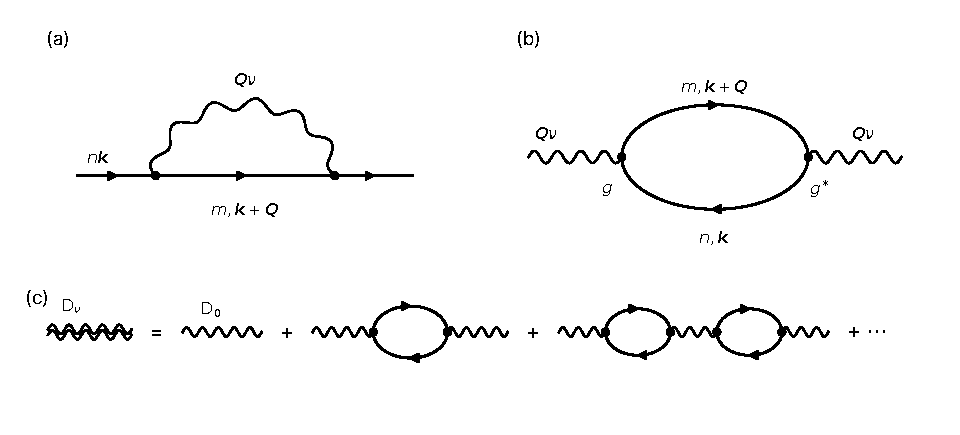
\includegraphics[width=\linewidth]{figures/ch06/fig6_5.pdf}
  \caption{The two second-order diagrams of the electron--phonon interaction. Solid lines with arrows are electrons, wavy lines phonons, dots the vertex $g$. (a) The electron self-energy: an electron in $(n,\vect{k})$ exchanges a phonon $(\vect{Q},\nu)$ with the intermediate state $(m,\vect{k}+\vect{Q})$. (b) The phonon self-energy: a phonon creates an electron in $(m,\vect{k}+\vect{Q})$ and a hole in $(n,\vect{k})$ through $g$, and the pair recombines through $g^*$. (c) The Dyson series for the dressed phonon propagator $\mathsf{D}_\nu$ (double wavy line): the free propagator $\mathsf{D}_0$ with any number of bubbles inserted.}
  \label{fig:6-bubble}
\end{figure}

The phonon Green's function in imaginary time is $\mathsf{D}_\nu(\vect{Q},\tau) = -\langle\mathrm{T}_\tau\,B_{\vect{Q}\nu}(\tau)\,B_{-\vect{Q}\nu}(0)\rangle$, with the free form $\mathsf{D}_0(\vect{Q}\nu,\ii\omega^{\mathrm{B}}_j) = 2\omega_{\vect{Q}\nu}/[(\ii\omega^{\mathrm{B}}_j)^2 - \omega_{\vect{Q}\nu}^2]$ of \cref{eq:D.11-D0}. Its expansion in $H_{\mathrm{ep}}$ is \cref{eq:D.11-Gexp} with $B_{\vect{Q}\nu}$ and $B_{-\vect{Q}\nu}$ as the external operators. The first nonzero correction is of second order. The expansion supplies $(-1)^2/2!$. The external $B_{\vect{Q}\nu}(\tau)$ is contracted with the boson of one of the two factors $H_{\mathrm{ep}}$, and $B_{-\vect{Q}\nu}(0)$ with the other; the two choices are equal after relabeling and cancel the $1/2!$. Each boson contraction is $-\mathsf{D}_0$. The vertex at $\tau_1$ must carry $B_{-\vect{Q}\nu}$, and the one at $\tau_2$ carries $B_{\vect{Q}\nu}$, so the vertices are $g_{mn\nu}(\vect{k},\vect{Q})^*$ and $g_{mn\nu}(\vect{k},\vect{Q})$ by \cref{eq:A.6-herm}, with the factor $1/N$ from the two $1/\sqrt N$. The two electron bilinears close into one loop, which gives $-1$ (rule 3 of \cref{app:D.11}) and a sum over two spin orientations. With the $-1$ of the definition, the total sign is $(-1)(-1)^2(-1) = +1$. In frequency space the correction is $\mathsf{D}_0\,\Pi^{\mathrm{b}}\,\mathsf{D}_0$ with
\begin{equation*}
  \Pi^{\mathrm{b}}_\nu(\vect{Q},\ii\omega^{\mathrm{B}}_j) = \frac2N\sum_{\vect{k}mn}|g_{mn\nu}(\vect{k},\vect{Q})|^2\;T\sum_{j'}\GF_0(n,\vect{k},\ii\omega^{\mathrm{F}}_{j'})\,\GF_0(m,\vect{k}+\vect{Q},\ii\omega^{\mathrm{F}}_{j'} + \ii\omega^{\mathrm{B}}_j) .
\end{equation*}
The frequency sum is \cref{eq:D.10-sum} with band labels, and
\begin{equation*}
  \Pi^{\mathrm{b}}_\nu(\vect{Q},\ii\omega^{\mathrm{B}}_j) = \frac2N\sum_{\vect{k}mn}|g_{mn\nu}(\vect{k},\vect{Q})|^2\,\frac{f_{n\vect{k}} - f_{m,\vect{k}+\vect{Q}}}{\ii\omega^{\mathrm{B}}_j + \varepsilon_{n\vect{k}} - \varepsilon_{m,\vect{k}+\vect{Q}}} .
\end{equation*}
Repeating the bubble along the phonon line gives the geometric series of \cref{fig:6-bubble}(c), $\mathsf{D} = \mathsf{D}_0 + \mathsf{D}_0\Pi^{\mathrm{b}}\mathsf{D}_0 + \dots = \mathsf{D}_0 + \mathsf{D}_0\Pi^{\mathrm{b}}\mathsf{D}$, so that $\mathsf{D}^{-1} = \mathsf{D}_0^{-1} - \Pi^{\mathrm{b}}$, a Dyson equation like \cref{eq:4.7-dyson} for electrons. With $\mathsf{D}_0^{-1} = [(\ii\omega^{\mathrm{B}}_j)^2 - \omega_{\vect{Q}\nu}^2]/2\omega_{\vect{Q}\nu}$ it is natural to define the self-energy in units of a squared frequency, $\Pi_\nu = 2\omega_{\vect{Q}\nu}\Pi^{\mathrm{b}}_\nu$. Continuing to $\omega + \ii0^+$,
\begin{keyresult}[Phonon self-energy and Dyson equation]
\begin{gather}
  \mathsf{D}_\nu(\vect{Q},\omega) = \frac{2\omega_{\vect{Q}\nu}}{\omega^2 - \omega_{\vect{Q}\nu}^2 - \Pi_\nu(\vect{Q},\omega)} , \notag\\
  \Pi_\nu(\vect{Q},\omega) = \frac{4\omega_{\vect{Q}\nu}}{N}\sum_{\vect{k}mn}|g_{mn\nu}(\vect{k},\vect{Q})|^2\,\frac{f_{n\vect{k}} - f_{m,\vect{k}+\vect{Q}}}{\omega + \varepsilon_{n\vect{k}} - \varepsilon_{m,\vect{k}+\vect{Q}} + \ii0^+} ,
  \label{eq:6.4-Pi}
\end{gather}
\end{keyresult}
with $f_{n\vect{k}} = n_{\mathrm{F}}(\xi_{n\vect{k}})$ the occupations and $\Pi_\nu$ in eV$^2$. The factor 4 is the 2 of $\mathsf{D}_0^{-1}$ times the two spin orientations of the loop. Note that we have put the screened vertex $g$ at both ends, with noninteracting electrons between them. Strictly, one end should carry the bare vertex~\cite[Eqs.~(145) and~(146)]{giustino2017electron}, which matters for the static part only. We have dropped the bubbles that connect two branches $\nu \ne \nu'$ at the same $\vect{Q}$. They mix the modes, and they matter where two branches are nearly degenerate.

The poles of $\mathsf{D}_\nu$ are the dressed phonons, $\omega^2 = \omega_{\vect{Q}\nu}^2 + \Pi_\nu(\vect{Q},\omega)$. When $|\Pi_\nu| \ll \omega_{\vect{Q}\nu}^2$ the root lies close to $\omega_{\vect{Q}\nu}$. Expanding the denominator there, $\omega^2 - \omega_{\vect{Q}\nu}^2 \simeq 2\omega_{\vect{Q}\nu}(\omega - \omega_{\vect{Q}\nu})$, turns $\mathsf{D}_\nu$ into a Lorentzian, $1/(\omega - \tilde\omega_{\vect{Q}\nu} + \ii\gamma_{\vect{Q}\nu}/2)$, with
\begin{equation}
  \tilde\omega_{\vect{Q}\nu} = \omega_{\vect{Q}\nu} + \frac{\Real\Pi_\nu(\vect{Q},\omega_{\vect{Q}\nu})}{2\omega_{\vect{Q}\nu}} , \qquad
  \gamma_{\vect{Q}\nu} = -\frac{\Imag\Pi_\nu(\vect{Q},\omega_{\vect{Q}\nu})}{\omega_{\vect{Q}\nu}} .
  \label{eq:6.4-pole}
\end{equation}
The real part shifts the phonon, and the imaginary part gives it a full width at half maximum $\gamma_{\vect{Q}\nu}$, the quantity of \cref{sec:5.7}. Its electron--phonon part is $\gamma^{\mathrm{ep}}_{\vect{Q}\nu}$, and the anharmonic bubble of \cref{sec:5.7} adds $\gamma^{\mathrm{anh}}_{\vect{Q}\nu}$ to it.

The sign of the static part is fixed. In an insulator at $T = 0$, $f_{n\vect{k}} - f_{m,\vect{k}+\vect{Q}} = +1$ for $n$ occupied and $m$ empty, and then $\varepsilon_{n\vect{k}} - \varepsilon_{m,\vect{k}+\vect{Q}} < 0$; the term with the roles exchanged has both signs reversed. Every term of $\Pi_\nu(\vect{Q},0)$ is therefore negative. The virtual pairs soften the lattice, as second-order perturbation theory always lowers a ground-state energy. In a metal the static bubble inherits the structure of the Lindhard function (\cref{sec:4.5}). For a spherical Fermi surface the density of pairs with $\varepsilon_{n\vect{k}} = \varepsilon_{m,\vect{k}+\vect{Q}} = E_{\mathrm{F}}$ changes abruptly when $Q$ passes $2k_{\mathrm{F}}$, the largest wavevector that joins two points of the surface, and the derivative of the Lindhard function diverges there logarithmically (\cref{app:C.8}). The phonon frequencies carry the singularity as a kink at $Q = 2k_{\mathrm{F}}$, or at whatever wavevectors span flat, parallel pieces of a real Fermi surface. This is the Kohn anomaly~\cite{kohn1959image}, and its position in a measured dispersion is an image of the Fermi surface.

\subsection{Adiabatic and nonadiabatic phonons}

The static part of $\Pi_\nu$ is already in the phonons we start from. Density-functional perturbation theory computes second derivatives of the Born--Oppenheimer energy with the electrons relaxed to their ground state at every nuclear configuration. The relaxation is the electronic response at zero frequency, which at this order is $\Pi_\nu(\vect{Q},0)$. The first-order density of \cref{eq:5.4-dn} is precisely that response, and the Hartree and exchange--correlation potential it generates is what turns the bare vertex at one end of the bubble into the screened one. Starting from the frequencies of such a calculation and adding the full $\Pi_\nu(\vect{Q},\omega)$ would count the static response twice. Only the difference between the dynamic and the static response may be added~\cite[Eqs.~(22) and~(23)]{calandra2010adiabatic},
\begin{equation}
  \bigl(\omega^{\mathrm{ren}}_{\vect{Q}\nu}\bigr)^2 = \omega_{\vect{Q}\nu}^2 + \Real\bigl[\Pi_\nu(\vect{Q},\omega^{\mathrm{ren}}_{\vect{Q}\nu}) - \Pi_\nu(\vect{Q},0)\bigr] ,
  \label{eq:6.4-nonad}
\end{equation}
where $\omega_{\vect{Q}\nu}$ is now the adiabatic frequency of density-functional perturbation theory and $\omega^{\mathrm{ren}}_{\vect{Q}\nu}$ the nonadiabatic one; this is the subtraction $W_e(\omega) - W_e(0)$ of Ref.~\cite[Eq.~(140)]{giustino2017electron}. The imaginary part needs no subtraction, since $\Pi_\nu(\vect{Q},0)$ is real.

How large is the remainder? In an insulator every denominator of \cref{eq:6.4-Pi} is at least $\Eg$ in magnitude, and the pair of terms with roles exchanged makes $\Pi_\nu$ even in $\omega$. The difference $\Pi_\nu(\omega) - \Pi_\nu(0)$ is then of relative order $(\omega_{\vect{Q}\nu}/\Eg)^2$, which is 0.003 for the optical phonon of silicon. The adiabatic phonons of an insulator are accurate, and this is the phonon-side statement of the counting of \cref{sec:6.1}, where $\omega_{\mathrm{ph}}/\Eg$ was the small parameter. A metal has no gap. Its intraband pairs with $|\varepsilon_{m,\vect{k}+\vect{Q}} - \varepsilon_{n\vect{k}}| \lesssim \omega_{\vect{Q}\nu}$ respond differently at $\omega = 0$ and at $\omega = \omega_{\vect{Q}\nu}$, and for them the difference is of order one. Such pairs dominate the bubble at small wavevector. For a band with Fermi velocity $v_{\mathrm{F}}$, the energy difference of a pair is $v_{\mathrm{F}}Q\cos\theta$, and the adiabatic and nonadiabatic frequencies differ appreciably only for $Q \lesssim \omega_{\vect{Q}\nu}/v_{\mathrm{F}}$~\cite{calandra2010adiabatic}. In aluminum, with $v_{\mathrm{F}} = \SI{2.0e6}{m.s^{-1}}$, that is $Q \lesssim \SI{2e-3}{\angstrom^{-1}}$ for a \SI{30}{meV} phonon, a thousandth of the zone. Near the zone center of metals with few carriers and stiff optical modes the correction can, however, be large. Calandra, Profeta and Mauri note corrections of up to \SI{30}{\percent} of the phonon frequency there~\cite{calandra2010adiabatic}; graphite intercalation compounds and doped graphene are the standard examples. Everywhere else the adiabatic frequencies are the right starting point.

The bubble with undressed vertices is itself an approximation. The counting of Migdal's theorem (\cref{sec:6.3}) makes the vertex corrections to it of relative order $\lambda_{\mathrm{ep}}\omega_{\mathrm{D}}/E_{\mathrm{F}}$, with the coupling constant $\lambda_{\mathrm{ep}}$ defined below; for aluminum, with phonon energies up to $\omega_{\max} = \SI{40}{meV}$ and $E_{\mathrm{F}} = \SI{11.7}{eV}$, that is at most 0.0015.

\subsection{The electron--phonon linewidth}

The width follows from the imaginary part of \cref{eq:6.4-Pi}. With $1/(x + \ii0^+) = \operatorname{PV}(1/x) - \ii\pi\delta(x)$ from \cref{eq:2.4-SP} in \cref{eq:6.4-pole},
\begin{keyresult}[Electron--phonon linewidth]
\begin{equation}
  \gamma^{\mathrm{ep}}_{\vect{Q}\nu} = -\frac{\Imag\Pi_\nu(\vect{Q},\omega_{\vect{Q}\nu})}{\omega_{\vect{Q}\nu}}
  = \frac{4\pi}{N}\sum_{\vect{k}mn}|g_{mn\nu}(\vect{k},\vect{Q})|^2\,\bigl(f_{n\vect{k}} - f_{m,\vect{k}+\vect{Q}}\bigr)\,\delta\bigl(\varepsilon_{m,\vect{k}+\vect{Q}} - \varepsilon_{n\vect{k}} - \omega_{\vect{Q}\nu}\bigr) ,
  \label{eq:6.4-gamma}
\end{equation}
\end{keyresult}
a full width, with the spin sum in the factor $4\pi = 2\times2\pi$. Ref.~\cite[Eq.~(146)]{giustino2017electron} writes the same rate as an inverse lifetime, with the spin factor 2 written explicitly, and its $1/\tau$ equals $\gamma^{\mathrm{ep}}_{\vect{Q}\nu}$. The cutting rule of \cref{sec:4.8} tells us how to read it. The delta function puts the pair on shell with the energy of the phonon, and $2\pi|g|^2/N$ times it is the golden-rule rate \cref{eq:2.5-golden} for absorbing the phonon into the pair $(n\vect{k} \to m,\vect{k}+\vect{Q})$. The occupation factor is the rate of that process, $f_n(1 - f_m)$, minus the rate of the inverse one, $f_m(1 - f_n)$, in which a pair recombines and emits the phonon; the difference is $f_n - f_m$.

In an undoped insulator at $T = 0$ the width vanishes below the gap. The delta function needs an occupied state $n$ and an empty state $m$ with $\varepsilon_m - \varepsilon_n = \omega_{\vect{Q}\nu}$, and every such difference is at least $\Eg$, while the largest phonon energy of silicon is \SI{64}{meV}. No term survives. The phonons of an insulator are, however, still broadened, by anharmonicity (\cref{sec:5.7}) and by isotopes and defects (\cref{sec:11.6}), which is why the measured \SI{0.18}{meV} width of the silicon Raman line could be compared with the three-phonon formula alone. At $T > 0$ thermally excited electrons and holes absorb phonons by intraband transitions, with a width proportional to their density, which in an intrinsic crystal is suppressed by $\ee^{-\Eg/2T}$: $4\times10^{-10}$ in silicon at room temperature. Doping supplies such carriers without the exponential, and a doped semiconductor behaves for this purpose like a dilute metal.

In a metal the electronic states near the Fermi level change on scales of eV, far larger than $\omega_{\vect{Q}\nu}$. For $T \ll E_{\mathrm{F}}$ the occupation difference at $\varepsilon_m = \varepsilon_n + \omega_{\vect{Q}\nu}$ is $f(\varepsilon_n) - f(\varepsilon_n + \omega_{\vect{Q}\nu}) \simeq -\omega_{\vect{Q}\nu}\,\partial f/\partial\varepsilon$, which tends to $\omega_{\vect{Q}\nu}\delta(\xi_{n\vect{k}})$ for $T \to 0$, and dropping $\omega_{\vect{Q}\nu}$ also in the remaining delta function, we arrive at Allen's formula~\cite{allen1972neutron},
\begin{equation}
  \gamma^{\mathrm{ep}}_{\vect{Q}\nu} \simeq \frac{4\pi\omega_{\vect{Q}\nu}}{N}\sum_{\vect{k}mn}|g_{mn\nu}(\vect{k},\vect{Q})|^2\,\delta(\xi_{n\vect{k}})\,\delta(\xi_{m,\vect{k}+\vect{Q}}) ,
  \label{eq:6.4-allen}
\end{equation}
which is positive term by term. Both electrons now sit on the Fermi surface, and the width is proportional to the phonon frequency. It no longer depends on temperature: thermal smearing removes states from below the Fermi level and adds them above, and the net number of pairs that can absorb $\omega_{\vect{Q}\nu}$ stays the same. The approximation requires bands that are smooth on the scale of $\omega_{\vect{Q}\nu}$ and a temperature small on the electronic scale. It fails for a band edge within $\omega_{\vect{Q}\nu}$ of the Fermi level, and for $Q \lesssim \omega_{\vect{Q}\nu}/v_{\mathrm{F}}$, the same small-$Q$ region where the nonadiabatic correction lives.

The electron gas makes the passage from \cref{eq:6.4-gamma} to \cref{eq:6.4-allen} explicit. For one parabolic band and a constant vertex, the angular integral in $(1/\Vol)\sum_{\vect{k}}(f_{\vect{k}} - f_{\vect{k}+\vect{Q}})\,\delta(\varepsilon_{\vect{k}+\vect{Q}} - \varepsilon_{\vect{k}} - \omega)$ gives $m_e/(kQ)$ wherever the delta function can be satisfied, and with $k\,\dd k = m_e\,\dd\varepsilon$ the radial integral becomes $\int\dd\varepsilon\,[f(\varepsilon) - f(\varepsilon + \omega)] = \omega$. The result, $m_e^2\omega/(4\pi^2Q)$ per spin and volume, holds at any $T \ll E_{\mathrm{F}}$ for $2k_{\mathrm{F}} > Q \gg \omega/v_{\mathrm{F}}$, and it is exactly what the double delta function of \cref{eq:6.4-allen} gives, $\omega\int\dd^3k\,(2\pi)^{-3}\delta(\xi_{\vect{k}})\,\delta(\xi_{\vect{k}+\vect{Q}}) = m_e^2\omega/(4\pi^2Q)$.

\subsection{The Eliashberg function}

The double sum in \cref{eq:6.4-allen} is a Fermi-surface average of $|g|^2$ for one phonon. Superconductivity, the electron mass enhancement and the resistivity of a metal all involve the same average, weighted over all phonons at a given energy. This weighted average is the Eliashberg function~\cite{eliashberg1960interactions},
\begin{equation}
  \alpha^2F(\omega) = \frac{1}{\mathcal{N}_{\mathrm{F}}\Omega\,N^2}\sum_{\vect{k}\vect{Q}}\sum_{mn\nu}|g_{mn\nu}(\vect{k},\vect{Q})|^2\,\delta(\xi_{n\vect{k}})\,\delta(\xi_{m,\vect{k}+\vect{Q}})\,\delta(\omega - \omega_{\vect{Q}\nu}) ,
  \label{eq:6.4-a2F}
\end{equation}
with $\mathcal{N}_{\mathrm{F}}$ the density of states per spin and volume at the Fermi level (\cref{sec:2.5}), so that $\mathcal{N}_{\mathrm{F}}\Omega$, per spin and per cell, satisfies $N\mathcal{N}_{\mathrm{F}}\Omega = \sum_{n\vect{k}}\delta(\xi_{n\vect{k}})$. The prefactor makes $\alpha^2F$ an average over initial states on the Fermi surface and a sum over final states, and it is dimensionless~\cite[Eq.~(205)]{giustino2017electron}. The symbol is read as one. If $|g|^2$ were the same for every pair on the Fermi surface, $\alpha^2F$ would be that constant times $\mathcal{N}_{\mathrm{F}}\Omega$ times the phonon density of states $g_{\mathrm{ph}}(\omega)$ of \cref{eq:5.2-dos}. The historical notation splits it this way into a coupling $\alpha^2(\omega)$ and a density $F(\omega)$. Comparing \cref{eq:6.4-allen,eq:6.4-a2F} term by term turns the Eliashberg function into a sum of linewidths, and it defines the coupling constant as its inverse moment~\cite[Eq.~(206)]{giustino2017electron}:
\begin{keyresult}[Eliashberg function, coupling constant and linewidths]
\begin{equation}
  \begin{gathered}
  \alpha^2F(\omega) = \frac{1}{4\pi\mathcal{N}_{\mathrm{F}}\Omega\,N}\sum_{\vect{Q}\nu}\frac{\gamma^{\mathrm{ep}}_{\vect{Q}\nu}}{\omega_{\vect{Q}\nu}}\,\delta(\omega - \omega_{\vect{Q}\nu}), \\
  \lambda_{\mathrm{ep}} = 2\int_0^\infty\dd\omega\,\frac{\alpha^2F(\omega)}{\omega} = \frac{1}{2\pi\mathcal{N}_{\mathrm{F}}\Omega\,N}\sum_{\vect{Q}\nu}\frac{\gamma^{\mathrm{ep}}_{\vect{Q}\nu}}{\omega_{\vect{Q}\nu}^2} .
  \end{gathered}
  \label{eq:6.4-lambda}
\end{equation}
\end{keyresult}
With a full width and a density of states per spin the factors are as written; a half width~\cite[Eq.~(185)]{giustino2017electron} or a two-spin $\mathcal{N}_{\mathrm{F}}$ changes them by factors of two. The coupling constant is a zone average of mode contributions $\lambda_{\vect{Q}\nu} = \gamma^{\mathrm{ep}}_{\vect{Q}\nu}/(2\pi\mathcal{N}_{\mathrm{F}}\Omega\,\omega_{\vect{Q}\nu}^2)$. We can therefore read the coupling of a mode off its measured linewidth, which was the point of Allen's relation~\cite{allen1972neutron}, and the factor $1/\omega^2$ makes soft modes with large widths dominate.

The name ``coupling constant'' comes from the electrons. Average the Fan--Migdal self-energy \cref{eq:6.3-FM} of a state $(n,\vect{k})$ over the Fermi surface, and insert $1 = \int\dd\omega'\,\delta(\omega' - \omega_{\vect{Q}\nu})\int\dd\varepsilon\,\delta(\varepsilon - \xi_{m,\vect{k}+\vect{Q}})$. Suppose that the density of final states and the vertices change little over the energy range $\omega_{\mathrm{D}}$ of the phonons. Then $\delta(\varepsilon - \xi_{m,\vect{k}+\vect{Q}})$ may be replaced by $\delta(\xi_{m,\vect{k}+\vect{Q}})$ under the average, and the weight of each $(\omega',\varepsilon)$ is $\alpha^2F(\omega')$ by \cref{eq:6.4-a2F}:
\begin{equation*}
  \langle\Sigma^{\mathrm{FM}}\rangle_{\mathrm{FS}}(\omega) = \int_0^\infty\dd\omega'\,\alpha^2F(\omega')\int_{-E_{\mathrm{band}}}^{E_{\mathrm{band}}}\dd\varepsilon\left[\frac{n_{\mathrm{B}}(\omega') + 1 - n_{\mathrm{F}}(\varepsilon)}{\omega - \varepsilon - \omega' + \ii0^+} + \frac{n_{\mathrm{B}}(\omega') + n_{\mathrm{F}}(\varepsilon)}{\omega - \varepsilon + \omega' + \ii0^+}\right] ,
\end{equation*}
where the cutoff $E_{\mathrm{band}} \gg \omega_{\mathrm{D}}$ is of the order of the band width. At $T = 0$ only $1 - \Theta(-\varepsilon) = \Theta(\varepsilon)$ survives in the first numerator and $\Theta(-\varepsilon)$ in the second. The $\varepsilon$ integrals are logarithms, $-\ln[(E_{\mathrm{band}} + \omega' - \omega)/(\omega' - \omega)]$ and $\ln[(E_{\mathrm{band}} + \omega' + \omega)/(\omega' + \omega)]$, whose derivatives at $\omega = 0$ are $-1/\omega' + 1/(E_{\mathrm{band}} + \omega')$ each and tend to $-1/\omega'$ for $E_{\mathrm{band}} \to \infty$; a finite band reduces each by the fraction $\omega'/(E_{\mathrm{band}} + \omega')$, \SI{1}{\percent} for $E_{\mathrm{band}} = 100\,\omega'$. The Allen--Heine term of \cref{eq:6.3-AH} does not depend on $\omega$ and does not contribute. The slope at the Fermi level is therefore $-2\int_0^\infty\dd\omega'\,\alpha^2F(\omega')/\omega'$, and by \cref{eq:6.4-lambda}
\begin{equation}
  -\frac{\partial\Real\langle\Sigma^{\mathrm{FM}}\rangle_{\mathrm{FS}}}{\partial\omega}\bigg|_{\omega=0} = \lambda_{\mathrm{ep}} .
  \label{eq:6.4-mass}
\end{equation}
By \cref{eq:4.7-qp} the quasiparticles within about $\omega_{\mathrm{D}}$ of the Fermi level have the residue $z_{\mathrm{qp}} = 1/(1 + \lambda_{\mathrm{ep}})$, their velocity is reduced by the same factor, and their density of states, and with it the electronic specific heat, is enhanced by $1 + \lambda_{\mathrm{ep}}$. The free electron gas has the specific heat $(\pi^2/3)\,2\mathcal{N}_{\mathrm{F}}\,T$ per volume~\cite[Chap.~2]{ashcroft1976solid}. For aluminum, for example, a density of states $2\mathcal{N}_{\mathrm{F}}\Omega = 5.49$ states per Ry and cell for both spins, computed from first principles~\cite[Table~II]{savrasov1996electron}, corresponds to \SI{0.951}{mJ.K^{-2}.mol^{-1}}, while the measured coefficient is \SI{1.36}{mJ.K^{-2}.mol^{-1}}~\cite[Table~II]{savrasov1996electron}. The ratio is $1 + \lambda_{\mathrm{ep}} = 1.43$. The specific heat alone measures $\lambda_{\mathrm{ep}} = 0.43$, without any phonon calculation.

The Eliashberg function has a different shape from the phonon density of states, and \cref{fig:6-a2F} shows by how much for aluminum. The model behind it is the simplest that still has the right ingredients. The phonons come from force constants between first and second neighbors of the fcc lattice, with $a = \SI{4.05}{\angstrom}$ and $M = \SI{26.98}{u}$. A neighbor at the lattice vector $\vect{R}$ contributes its spring tensor times $1 - \cos(\vect{Q}\cdot\vect{R})$ to the dynamical matrix, divided by $M$. The tensor of the first neighbor at $(a/2)(1,1,0)$ has the elements $0.648$ ($xx = yy$), $-0.187$ ($zz$) and $0.574$ ($xy$), and that of the second neighbor at $a(1,0,0)$ has $0.038$ ($xx$) and $-0.052$ ($yy = zz$), all in \si{eV.\angstrom^{-2}}. These five numbers are a least-squares fit to the measured zone-boundary frequencies, 9.69 and \SI{5.78}{THz} (longitudinal and transverse) at X and 9.69 and \SI{4.19}{THz} at L~\cite[Table~I]{savrasov1996electron}, and to the elastic constants $C_{11} = 106.8$, $C_{12} = 60.7$ and $C_{44} = \SI{28.2}{GPa}$ at a density of \SI{2.70}{g.cm^{-3}}~\cite{kittel2005introduction}, the room-temperature values of that source. They reproduce the transverse frequencies at X and L to \SI{2}{\percent} and the longitudinal one at L to \SI{8}{\percent}, and the largest phonon energy is \SI{40}{meV}.

The electrons are a free gas of three electrons per atom, with $k_{\mathrm{F}} = \SI{1.75}{\angstrom^{-1}}$ and $E_{\mathrm{F}} = \SI{11.7}{eV}$. The potential of each ion is a Coulomb potential $-3e^2/(4\pi r)$ outside a core radius $r_{\mathrm{c}}$ and zero inside, screened by the Lindhard function of \cref{sec:4.5}. Its Fourier transform per cell is $w(q) = -3e^2\cos(qr_{\mathrm{c}})/[\Omega q^2\varepsilon_{\mathrm{Lin}}(q,0)]$. For plane waves and one atom per cell, \cref{eq:A.6-g} becomes $g_\nu = (2M\omega_{\vect{Q}\nu})^{-1/2}(\vect{q}\cdot\vect{e}_\nu)\,w(q)$, where $\vect{q} = \vect{Q} + \vect{G}$ is the full momentum transfer, umklapp included. The sums over $\vect{k}$ and over the reciprocal-lattice vectors become integrals, $N^{-1}\sum_{\vect{k}} \to \Omega\int\dd^3k/(2\pi)^3$ and $N^{-1}\sum_{\vect{Q}}\sum_{\vect{G}} \to \Omega\int\dd^3q/(2\pi)^3$. The double delta function integrates to $\int\dd^3k\,(2\pi)^{-3}\delta(\xi_{\vect{k}})\delta(\xi_{\vect{k}+\vect{q}}) = m_e^2/(4\pi^2q)$ for $q < 2k_{\mathrm{F}}$, as for the linewidth of the electron gas, and with $\mathcal{N}_{\mathrm{F}} = m_ek_{\mathrm{F}}/2\pi^2$, \cref{eq:6.4-a2F} becomes
\begin{equation}
  \alpha^2F(\omega) = \frac{m_e\Omega}{2k_{\mathrm{F}}}\int_{q<2k_{\mathrm{F}}}\frac{\dd^3q}{(2\pi)^3}\sum_\nu\frac{(\hat{\vect{q}}\cdot\vect{e}_\nu)^2\,q\,|w(q)|^2}{2M\omega_{\vect{q}\nu}}\,\delta(\omega - \omega_{\vect{q}\nu}) .
  \label{eq:6.4-a2Fgas}
\end{equation}
The core radius is the only free parameter, a choice of the model. As a function of $r_{\mathrm{c}}$, $\lambda_{\mathrm{ep}}$ has a flat minimum at $r_{\mathrm{c}} = \SI{0.56}{\angstrom}$, where the zero of $\cos(qr_{\mathrm{c}})$ sits among the umklapp momentum transfers between $|\vect{G}_{111}| = \SI{2.69}{\angstrom^{-1}}$ and $2k_{\mathrm{F}} = \SI{3.50}{\angstrom^{-1}}$. We take $r_{\mathrm{c}}$ there, where the result depends least on it; between 0.55 and \SI{0.59}{\angstrom} the coupling stays between 0.44 and 0.46. The model uses no measured coupling.

\begin{figure}[t]
  \centering
  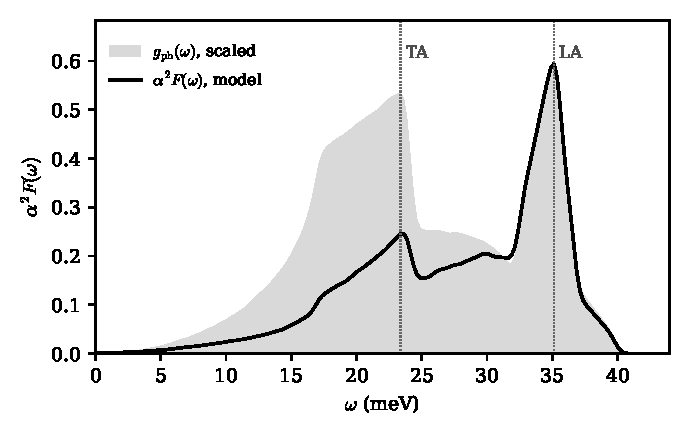
\includegraphics[width=0.75\linewidth]{figures/ch06/fig6_6.pdf}
  \caption{Eliashberg function of aluminum (black line) in a model of free electrons scattered by screened empty-core ions, \cref{eq:6.4-a2Fgas}, with the core radius, \SI{0.56}{\angstrom}, taken where $\lambda_{\mathrm{ep}}$ is stationary in it, with phonons from force constants between first and second neighbors fitted to measured zone-boundary frequencies and elastic constants. The gray area is the phonon density of states $g_{\mathrm{ph}}(\omega)$ of the same force constants, scaled to the height of the $\alpha^2F$ peak. Dotted lines mark the transverse (TA) and longitudinal (LA) maxima of $g_{\mathrm{ph}}$. In $\alpha^2F$ the transverse peak is suppressed, although three quarters of the modes lie below \SI{32}{meV}, because a transverse displacement couples to an electron only when the momentum transfer leaves the first zone. Both curves are histograms in bins of \SI{0.25}{meV} smoothed by a Gaussian of \SI{0.3}{meV}.}
  \label{fig:6-a2F}
\end{figure}

The result is $\lambda_{\mathrm{ep}} = 0.436$, against 0.44 from a linear-response calculation and 0.42 from tunneling spectra~\cite[Table~II]{savrasov1996electron}, and 0.43 from the specific heat above. Savrasov and Savrasov found their first-principles $\alpha^2F$ practically identical to an empirical rigid-ion pseudopotential result of this kind~\cite{savrasov1996electron}, and aluminum is the metal where the free-electron picture is expected to work. The shape carries more information than the number. Compared to the density of states, the transverse peak near \SI{23}{meV} is strongly suppressed. The reason is the factor $(\hat{\vect{q}}\cdot\vect{e}_\nu)^2$: within the first zone a transverse wave moves the ions perpendicular to $\vect{q}$, and an electron feels it only through an umklapp process, where $\vect{q} = \vect{Q} + \vect{G}$ has a component along the displacement. The logarithmic average frequency, $\omega_{\log} = \exp[(2/\lambda_{\mathrm{ep}})\int\dd\omega\,\alpha^2F(\omega)\ln\omega/\omega]$, which sets the prefactor of the critical temperature, comes out as \SI{250}{K}, against \SI{270}{K} from the linear-response calculation~\cite[Table~III]{savrasov1996electron}. A constant $\alpha^2$ with the same total weight would give 0.50 and \SI{228}{K}. Summed over the zone with \cref{eq:6.4-lambda}, the model widths average $\gamma^{\mathrm{ep}}_{\vect{Q}\nu}/\omega_{\vect{Q}\nu} = 4.4\times10^{-3}$ over all modes, or \SI{0.12}{meV}: a phonon in aluminum decays into electron--hole pairs after about 36 periods, much as the optical phonon of silicon decays anharmonically.

\begin{workedexample}{Coupling constant of aluminum from two Einstein peaks}\label{we:6-al}
Replace the model $\alpha^2F$ of \cref{fig:6-a2F} by two delta functions at the maxima of the phonon density of states, $\omega_{\mathrm{TA}} = \SI{23.4}{meV}$ and $\omega_{\mathrm{LA}} = \SI{35.1}{meV}$, each carrying the weight of $\alpha^2F$ on its side of the minimum of $g_{\mathrm{ph}}$ at \SI{31.9}{meV}. The weights are $I_{\mathrm{TA}} = \int_0^{31.9}\dd\omega\,\alpha^2F = \SI{3.13}{meV}$ and $I_{\mathrm{LA}} = \SI{2.26}{meV}$. Below the minimum lie 2.24 of the three modes per atom and above it 0.76, a ratio of 2.9; the weights of $\alpha^2F$ stand in the ratio 1.4, so each transverse mode couples half as strongly as a longitudinal one.

With $\alpha^2F = I_{\mathrm{TA}}\delta(\omega - \omega_{\mathrm{TA}}) + I_{\mathrm{LA}}\delta(\omega - \omega_{\mathrm{LA}})$, \cref{eq:6.4-lambda} gives
\begin{equation*}
  \lambda_{\mathrm{ep}} = 2\Bigl(\frac{I_{\mathrm{TA}}}{\omega_{\mathrm{TA}}} + \frac{I_{\mathrm{LA}}}{\omega_{\mathrm{LA}}}\Bigr) = 2\,(0.134 + 0.064) = 0.396 ,
\end{equation*}
\SI{9}{\percent} below the full model's 0.436 and 6 to \SI{8}{\percent} below the measured 0.42--0.43. The deficit is all in the transverse peak. The same weight spread over the low-frequency tail of \cref{fig:6-a2F} counts for more, since $1/\omega$ is convex, and the full transverse part is 0.306 instead of $2\times0.134 = 0.268$; the longitudinal part is 0.130 in both. Although the longitudinal peak is the taller, the transverse branches carry \SI{70}{\percent} of the coupling. For the two-peak model $\omega_{\log} = \exp[(2/\lambda_{\mathrm{ep}})(I_{\mathrm{TA}}\ln\omega_{\mathrm{TA}}/\omega_{\mathrm{TA}} + I_{\mathrm{LA}}\ln\omega_{\mathrm{LA}}/\omega_{\mathrm{LA}})] = \SI{26.7}{meV} = \SI{310}{K}$, too high for the same reason.
\end{workedexample}

In practice $\gamma^{\mathrm{ep}}_{\vect{Q}\nu}$ and $\alpha^2F$ are computed from \cref{eq:6.4-gamma,eq:6.4-a2F} with the vertices of density-functional perturbation theory, Wannier-interpolated to fine grids of $\vect{k}$ and $\vect{Q}$ as described in \cref{sec:6.2}. The two delta functions that pin both electrons to the Fermi surface make these the slowest-converging integrals of electron--phonon theory. \Cref{app:E.9} takes the resulting $\alpha^2F$ into the Eliashberg equations for the gap of aluminum, which come out at the measured \SI{0.18}{meV} once the Coulomb repulsion between paired electrons is fixed by the measured critical temperature.

The phonon-mediated attraction that binds those pairs is the exchange of the phonons whose widths we have just summed. \Cref{sec:7.2} reduces it to the model interaction of Bardeen, Cooper and Schrieffer, with $\lambda_{\mathrm{ep}}$ as its strength and $\omega_{\mathrm{D}}$ as its range in energy, and finds the gap that sets the threshold of a superconducting detector.
